\input{01-EtudeAeronefs/img/Cycle4Temps/ElementsMoteur.tex}

\section{Les groupes motopropulseurs}

	\subsection{Moteurs à pistons}
		\subsubsection{Description du moteur à piston}
		Le moteur à piston, également appelé moteur à combustion interne ou moteur à explosion est un moteur qui transforme l'énergie chimique contenue dans le carburant (essence, gasoil, gaz...) en énergie mécanique.
		\begin{figure}[H]
  		\centering
    		% INTAKE STROKE
\begin{tikzpicture}[scale=\echelleTikz]
  \def\d{-60}
  \engine{10};
  \draw[vector] (\d:.6*\R) arc (\d:\d-80:.55*\R);
  \fill[\gas]
    (VLo) to[out=110,in=0] ++ (-1.5,0.6) -- ($(VLo)+(-1.5,1.3)$) to[out=0,in=110] (VLm) to[out=\vl-90,in=\vl-90] cycle;
  \wall
  \valveL{.3}
  \valveR{.1}
  
  \draw[arrow] (VL) ++ (-.2,.2) --++ (-1,-.5)
    node[below left=-2,align=right,scale=1.4] {valve\\[-2pt]d'admission};
  \draw[arrow] (VR) ++ (.2,.1) --++ (1,-.5)
    node[below right=-2,align=left,scale=1.4] {valve\\[-2pt]d'échappement};
  \draw[arrow] (O) ++ (-.2,.4) --++ (-2.0,.9)
    node[left=-20,above left=2,scale=1.4] {villebrequin};
  \draw[arrow] (P) ++ (1.1,-.2) --++ (1.2,-.5)
    node[below right=-2,scale=1.4] {piston};
  \draw[arrow] (P) ++ (1.5,0.4) --++ (1.2,-.5)
    node[below right=-2,scale=1.4] {cylindre};
  \draw[arrow] (P) ++ (-1,0.97) --++ (-1.2,-.5);
  \draw[arrow] (P) ++ (-1,0.67) --++ (-1.2,-.2) %-0.5 - (0.97-0.67) = -0.2
    node[below left=-2,scale=1.4] {segments};
  \draw[arrow] (PL) ++ (2.2,-1.9) --++ (1.68,-.7)
    node[below right=-2,scale=1.4] {bielle};
  \draw[arrow] (O) ++ (-1.9,-0.8) --++ (-1.2,.5)
    node[left=-20,above left=2,scale=1.4] {carter};
  \draw[arrow] (S) ++ (150:.2) --++ (-.5,.7)
    node[above=-1,align=center,scale=1.4] {bougie};
  \draw[arrow] (VLm) ++ (-1.5,.5) --++ (-1.5,.7)
    node[above left=-2,align=right,scale=1.4] {pipe\\[-2pt]d'admission};
  \draw[arrow] (VRm) ++ (1.5,.5) --++ (1.5,.7)
    node[above right=-2,align=left,scale=1.4] {pipe\\[-2pt]d'échappement};
  
\end{tikzpicture}
  		\legende{Schéma d'un moteur à piston}{tikz:schemaMoteurPiston}
		\end{figure}
		
		Le moteur à piston est composé des éléments principaux suivants :
		\begin{itemize}
			\item cylindre
			\item piston : pièce mobile dans le cylindre
			\item bielle : pièce qui fait la jonction entre le cylindre et le vilebrequin
			\item vilebrequin : manivelle qui convertit le mouvement alternatif du piston en mouvement rotatif
			\item bougie : système d'allumage qui permet de commander la combustion du mélange contenu dans le cylindre
			\item soupape d'admission et d'échappement : pièces mobiles qui permettent de faire rentrer le mélange et de faire sortir les gaz d'échappement du cylindre 
			\item pipe d'admission et d'échappement : tubes qui permettent d'acheminer respectivement le mélange air-essence dans le réservoir et les gaz brûlés vers l'échappement
			\item carter : bas du moteur. Contient notamment l'huile nécessaire au fonctionnement du moteur
			\item segments : anneaux métalliques installés sur le cylindre. Assure l'étanchéité entre le piston et le cylindre.
		\end{itemize}
	
		\subsubsection{Le cycle à 4 temps}
		\renewcommand{\echelleTikz}{0.5}
		\paragraph{Admission}
		
		L'admission est le premier cycle du cycle à 4 temps. Durant cette phase, qui démarre alors que le piston est en point haut, la soupape d'admission s'ouvre. La descente du piston durant cette étape permet l'aspiration du mélange air-carburant dans le cylindre. Lorsque le cylindre atteint son point bas, la soupape d'admission est refermée.

		\begin{figure}[H]
  		\centering
    		% INTAKE STROKE
\def\gas{blue!50}
\begin{tikzpicture}[scale=\echelleTikz]
  \def\d{-60}
  \engine{10};
  %\draw[vector] (\d:.6*\R) arc (\d:\d-80:.55*\R);
  \fill[\gas, opacity=0.5]
    (VLo) to[out=110,in=0] ++ (-1.5,0.6) -- ($(VLo)+(-1.5,1.3)$) to[out=0,in=110] (VLm) to[out=\vl+5,in=\vl-47] cycle;
  \wall
  \valveL{.3}
  \valveR{.1};
  
\end{tikzpicture}
  		\legende{Étape 1 : Admission}{tikz:schemaMoteurPiston}
		\end{figure}	

		\paragraph{Compression}
		
		Dans ce deuxième cycle, qui débute alors que le piston est en position basse, les 2 soupapes sont fermées. Le piston remonte et le mélange air-carburant précédemment admis est comprimé dans le cylindre.
		
		\begin{figure}[H]
  		\centering
    		% COMPRESSION STROKE
\begin{tikzpicture}[scale=\echelleTikz]
  \def\d{-10}
  \engine{-140};
  \draw[vector] (\d:.6*\R) arc (\d:\d-80:.55*\R);
  \valveL{.1}
  \valveR{.1}
\end{tikzpicture}
  		\legende{Étape 2 : Compression}{tikz:schemaMoteurPiston}
		\end{figure}	
		
		\paragraph{Explosion-détente}
		
		Dans ce cycle, qui démarre alors que le piston atteint à nouveau le point haut, l'étincelle provoquée par la bougie provoque l'explosion du mélange présent dans le cylindre. Le piston est alors repoussé vers le bas. Durant ce cycle, les 2 soupapes restent fermées.
		
		\begin{figure}[H]
  		\centering
		% IGNITION
\begin{tikzpicture}[scale=\echelleTikz]
  \def\d{40}
  \engine{90};
  \draw[vector] (\d:.6*\R) arc (\d:\d-80:.55*\R);
  \valveL{.1}
  \valveR{.1}
  \draw[very thin,yellow!70!black,fill=yellow,shift={(X)}]
    ( -15:.20) -- ( -30:.40) -- ( -40:.25) -- ( -50:.40) --
    ( -60:.22) -- ( -70:.40) -- ( -80:.20) -- ( -90:.45) --
    (-100:.24) -- (-110:.40) -- (-120:.25) -- (-130:.40) --
    (-140:.20) -- (-150:.45) -- (-165:.20) to[out=40,in=140] cycle;
\end{tikzpicture}
  		\legende{Étape 3 : Explosion-détente}{tikz:schemaMoteurPiston}
		\end{figure}	
		
		\info{Le cycle d'explosion-détente est le seul cycle qui produit effectivement de l'énergie.}
		
		\paragraph{Échappement}
		
		Dans cette quatrième et dernière étape du cycle, la soupape d'échappement est ouverte. Le piston, initialement en point bas, remonte et pousse les gaz brûlés issus de la combustion en dehors du cylindre lors de la remontée. L'étape d'échappement se termine lorsque le piston atteint le point haut, la soupape d'échappement est alors refermée.
		
		\begin{figure}[H]
  		\centering
		% EXHAUST STROKE
\def\gas{blue!50}
\begin{tikzpicture}[scale=\echelleTikz]
  \def\d{-40}
  \engine{-190};
  \draw[vector] (\d:.6*\R) arc (\d:\d-80:.55*\R);
  \fill[\gas, opacity=0.5]
    (VRo) to[out=60,in=-180] ++ (1.5,0.6) -- ($(VRo)+(1.5,1.3)$) to[out=180,in=60] (VRm) to[out=-220+\vr,in=-180+\vr] cycle;
  \wall
  \valveL{.1}
  \valveR{.3}
\end{tikzpicture}
  		\legende{Étape 4 : Échappement}{tikz:schemaMoteurPiston}
		\end{figure}	
		
		\paragraph{Cycle complet}
		
		L'animation suivante permet de visualiser le fonctionnement d'un moteur à explosion.	
		
		\renewcommand{\echelleTikz}{0.5}
		\begin{figure}[H]
  		\centering
		% Définition des couleurs de base
\definecolor{gazFroid}{RGB}{173,216,230}     % Bleu clair
\definecolor{gazChaud}{RGB}{255,0,0}         % Rouge
\definecolor{gazExplosion}{RGB}{255,255,0}   % Jaune
\definecolor{gazBrule}{RGB}{128,128,128}     % Gris

% Définition des couleurs de base
\definecolor{gazFroid}{RGB}{173,216,230}     % Bleu clair
\definecolor{gazChaud}{RGB}{255,0,0}         % Rouge
\definecolor{gazExplosion}{RGB}{255,255,0}   % Jaune
\definecolor{gazBrule}{RGB}{128,128,128}     % Gris

% Définition de la couleur des gaz en fonction de l'angle
\newcommand{\setGasColor}[1]{%
    \def\angle{#1}%
    % De gris à bleu (-90 à -30)
    \ifnum\angle<-30
        \def\gas{gazBrule!\the\numexpr100-(((\angle+90)*100)/60)\relax!gazFroid}%
    \else
        % Bleu constant (-30 à 90)
        \ifnum\angle<90
            \def\gas{gazFroid}%
        \else
            % De bleu vers rouge (90 à 270)
            \ifnum\angle<270
                \def\gas{gazFroid!\the\numexpr100-((\angle-90)*100/180)\relax!gazChaud}%
            \else
                % De rouge vers jaune (270 à 300)
                \ifnum\angle<300
                    \def\gas{gazChaud!\the\numexpr((\angle-270)*100/30)\relax!gazExplosion}%
                \else
                    % De jaune vers gris (300 à 450)
                    \ifnum\angle<450
                        \def\gas{gazExplosion!\the\numexpr100-((\angle-300)*100/150)\relax!gazBrule}%
                    \else
                        % Gris constant (450 à 630)
                        \def\gas{gazBrule}%
                    \fi
                \fi
            \fi
        \fi
    \fi
}

\ifdefined\activeranimations 
\newcommand{\nbFramesMoteurAnime}{360}
\else
\newcommand{\nbFramesMoteurAnime}{1}
\fi

\begin{animateinline}[autoplay,loop,controls]{60}
\multiframe{\nbFramesMoteurAnime}{i=-90+2}{%
    \begin{tikzpicture}
    \setGasColor{\i}%
      \coordinate (boiteLegende1) at (0,8.5);
      \coordinate (boiteLegende2) at (0,9);
      \node[rectangle,minimum width=2cm] [fit = (boiteLegende1) (boiteLegende2)] (legende) {};    
    
      \engine{-\i}
      
      % INTAKE STROKE
      \ifnum\i>-92 \ifnum\i<-88 
          \node[align=center,font=\Large] at (legende.center) {\textbf{Admission}};
          \valveL{.2}
          \valveR{.1};
      \fi \fi 
      \ifnum\i>-90 \ifnum\i<90 
          \node[align=center,font=\Large] at (legende.center) {\textbf{Admission}};
          \setGasColor{\i}%
          \fill[\gas, opacity=0.5]
              (VLo) to[out=110,in=0] ++ (-1.5,0.6) -- ($(VLo)+(-1.5,1.3)$) to[out=0,in=110] (VLm) to[out=\vl+5,in=\vl-47] cycle;
          \wall
          \valveL{.3}
          \valveR{.1};
      \fi \fi
      
      % COMPRESSION STROKE
      \ifnum\i>90 \ifnum\i<272 
          \node[align=center,font=\Large] at (legende.center) {\textbf{Compression}};
          \valveL{.1}
          \valveR{.1};
      \fi \fi 
      
      % POWER STROKE
      \ifnum\i>270 \ifnum\i<452 
          \node[align=center,font=\Large] at (legende.center) {\textbf{Explosion-détente}};
          \valveL{.1}
          \valveR{.1};
      \fi \fi
      
      % EXHAUST STROKE
      \ifnum\i>452 \ifnum\i<630
          \node[align=center,font=\Large] at (legende.center) {\textbf{Echappement}};
          \fill[\gas, opacity=0.5]
              (VRo) to[out=60,in=-180] ++ (1.5,0.6) -- ($(VRo)+(1.5,1.3)$) to[out=180,in=60] (VRm) to[out=-220+\vr,in=-180+\vr] cycle;
          \wall 
          \valveL{.1}
          \valveR{.3};
      \fi \fi
      
      % IGNITION
      \ifnum\i>268 \ifnum\i<280 
          \draw[very thin,yellow!70!black,fill=yellow,shift={(X)}]
              ( -15:.20) -- ( -30:.40) -- ( -40:.25) -- ( -50:.40) --
              ( -60:.22) -- ( -70:.40) -- ( -80:.20) -- ( -90:.45) --
              (-100:.24) -- (-110:.40) -- (-120:.25) -- (-130:.40) --
              (-140:.20) -- (-150:.45) -- (-165:.20) to[out=40,in=140] cycle; 
      \fi \fi 
    \end{tikzpicture}
  }
\end{animateinline}
  		\legende{Le fonctionnement d'un moteur à explosion (animé)}{tikz:schemaMoteurPistonAnime}
		\end{figure}	
		
	\subsubsection{Nombre et disposition des cylindres}
	Pour augmenter la puissance et la régularité de fonctionnement, la plupart des moteurs à pistons sont dôtés de plusieurs cylindres. Ce nombre va de 1 à 28 cylindres pour les plus gros moteurs.
	
	Dans l'histoire des moteurs à pistons, les concepteurs de ces moteurs ont testé de nombreuses dispositions. Chacune a ses forces et ses faiblesses, nous listerons ici quelques unes des dispositions les plus courantes parmi les dispositions que l'on trouve dans l'aéronautique.
	
	\paragraph{Cylindres en ligne}
	
	Une des disposition "évidente" pour un moteur à plusieurs cylindres : les cylindres sont disposés alignés les uns à la suite des autres.
	
	Cette simplicité apporte cependant plusieurs inconvénients :
	\begin{itemize}
		\item la disposition impose un moteur monté "débout", ce qui va imposer un capot relativement haut qui peut générer la visibilité vers l'avant, notamment au sol,
		\item un refroidissement peu efficace en raison de l'alignement des 4 cylindres : si le premier sera bien refroidi, les suivants verront passer un air d'autant plus réchauffé que l'on s'éloignera de l'avant du moteur.
	\end{itemize}

	\begin{center}
		\begin{minipage}[c]{1.0\linewidth}
		\begin{figure}[H]
		\begin{minipage}[c]{0.3\linewidth}
		\centering
		\includegraphics[width=0.8\textwidth]{01-EtudeAeronefs/img/flat4.png}
  		\legende{Moteur en ligne 4 cylindres}{video:flat4}
		\end{minipage}
		\begin{minipage}[c]{0.7\linewidth}
		\centering
		\includegraphics[width=0.95\linewidth]{01-EtudeAeronefs/img/renault4P.png}
		\legende{Un moteur d'avion en ligne Renault 4P}{img:renault4P}
		\end{minipage}
		\end{figure}
		\end{minipage}
	\end{center}	
	
	\paragraph{Moteur à plat}
	\begin{figure}[H]
  		\centering
    		
	\end{figure}	
	
	\begin{center}
		\begin{minipage}[c]{1.0\linewidth}
		\begin{figure}[H]
		\begin{minipage}[c]{0.5\linewidth}
		\centering
		\includegraphics[width=0.95\textwidth]{01-EtudeAeronefs/img/boxer4.png}
  		\legende{Moteur à plat 4 cylindres}{video:boxer4}
		\end{minipage}
		\begin{minipage}[c]{0.5\linewidth}
		\centering
		\includegraphics[width=0.95\linewidth]{01-EtudeAeronefs/img/boxer6.jpg}
		\legende{Un moteur d'avion à plat 6 cylindres Lycoming GO480}{img:boxer6}
		\end{minipage}
		\end{figure}
		\end{minipage}
	\end{center}
	
	\paragraph{Moteur en étoile}
	Le moteur en étoile \anglais{radial engine} a été très utilisée dans l'aviation. En effet, il présente de nombreux avantages dans une utilisation aéronautique :
	\begin{itemize}
		\item refroidissement : tous les cylindres sont exposés de façon identique au flux d'air de refroidissement
		\item compacité et légèreté
		\item système de graissage naturellement adapté à une utilisation "toute position" et donc à la voltige
	\end{itemize}
	
	\info{Les moteurs en étoile sont toujours équipés d'un nombre impair de cylindres.}
	
	\begin{figure}[H]
  		\centering
    		\includegraphics[width=0.5\textwidth]{01-EtudeAeronefs/img/5cylindresEtoile.png}
  		\legende{Moteur en étoile 5 cylindres}{video:5CylindresEtoile}
	\end{figure}	
	\begin{figure}[H]
  		\centering
    		
	\end{figure}	
	
	\begin{center}
		\begin{minipage}[c]{1.0\linewidth}
		\begin{figure}[H]
		\begin{minipage}[c]{0.5\linewidth}
		\centering
		\includegraphics[width=0.95\textwidth]{01-EtudeAeronefs/img/9cylindresEtoile.png}
  		\legende{Moteur en étoile 9 cylindres (illustration)}{video:9CylindresEtoile}
		\end{minipage}
		\begin{minipage}[c]{0.5\linewidth}
		\centering
		\includegraphics[width=0.95\linewidth]{01-EtudeAeronefs/img/PWWasp.jpg}
		\legende{Un moteur d'avion en étoile 9 cylindres, Pratt \& Whitney Wasp}{img:PWWasp}
		\end{minipage}
		\end{figure}
		\end{minipage}
	\end{center}
	
	\astuce{Il existe des moteurs en étoile avec un nombre paire de cylindres. Il s'agit en fait de moteurs qui sont composés de plusieurs moteurs en étoile couplés. Par exemple, Pratt \& Whitney a ainsi conçu des moteurs en étoile à 18 cylindres (2 étages de 9 cylindres) ou 28 cylindres (4 étages de 7 cylindres).}
	
	\paragraph{Moteur en V}
	\begin{figure}[H]
  		\centering
    		
	\end{figure}	
	
	\begin{center}
		\begin{minipage}[c]{1.0\linewidth}
		\begin{figure}[H]
		\begin{minipage}[c]{0.5\linewidth}
		\centering
		\includegraphics[width=0.95\textwidth]{01-EtudeAeronefs/img/v6.png}
  		\legende{Moteur en V 6 cylindres (V6)}{video:v6}
		\end{minipage}
		\begin{minipage}[c]{0.5\linewidth}
		\centering
		\includegraphics[width=0.95\linewidth]{01-EtudeAeronefs/img/moteurV12.jpg}
		\legende{Un moteur V12 aéronautique (1940)}{img:moteurV12}
		\end{minipage}
		\end{figure}
		\end{minipage}
	\end{center}
	
	\paragraph{Moteur rotatif}
	
	\begin{figure}[H]
  		\centering
    		\includegraphics[width=0.3\textwidth]{01-EtudeAeronefs/img/rotatif.png}
  		\legende{Moteur rotatif}{video:rotatif}
	\end{figure}	
	
	\subsubsection{Système d'allumage}
	
	\begin{figure}[H]
  		\centering
    		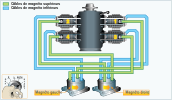
\includegraphics[width=0.5\textwidth]{01-EtudeAeronefs/img/systemesAvion/systemeAllumage.pdf}
  		\legende{Système d'allumage sur un moteur à 4 cylindres à plat)}{img:systemeAllumage}
	\end{figure}	
	
	\subsubsection{Système d'alimentation en carburant}
	
	Pour fonctionner, un moteur à combustion interne nécessite d'être alimenté par un mélange d'air et d'essence dans un rapport d'environ $1/15^{ième}$ (quinze gramme d'air pour 1 gramme d'essence). Ce rapport est nécessaire pour assurer un mélange st\oe chiométrique\footnote{Le mélange st\oe chiométrique pour un moteur à essence est le rapport idéal air/carburant qui brûle tout le carburant sans excès d'air.}, c'est à dire que le quantité d'oxygène admise dans le cylindre soit suffisante pour assurer la combustion complète du carburant qui l'accompagne. La combustion totale permet d'optimiser la consommation de carburant en extrayant le maximum d'énergie, mais également d'éviter un encrassement du moteur par la production de suies et autres dépôts qui accompagnent toujours une combustion incomplète.
	
	Dans un moteur, cette fonction peut être assurée par un carburateur ou un système d'injection. Sur beaucoup d'avion, on a encore recours assez largement aux carburateurs, bien que les systèmes d'injection tendent à se généraliser.
	
	\paragraph{Le carburateur}
	
	Sur un carburateur, le papillon est commandé directement par la manette des gaz. Lorsque le papillon est fermé, la quantité de carburant aspiré est faible, ce qui réduit le régime de rotation du moteur. La pleine ouverte du papillon va au contraire permettre l'admission d'une grande quantité de mélange dans les cylindres.
	
	Le carburateur est notamment composé d'un tube venturi. Dans cette portion du carburateur, on réduit la section disponible pour le passage de l'air. Cela provoque, par effet Venturi, une accélération et une dépression, ce qui va permettre d'aspirer et de vaporiser le carburant présent au niveau du gicleur.
	
	\begin{figure}[H]
  		\centering
    		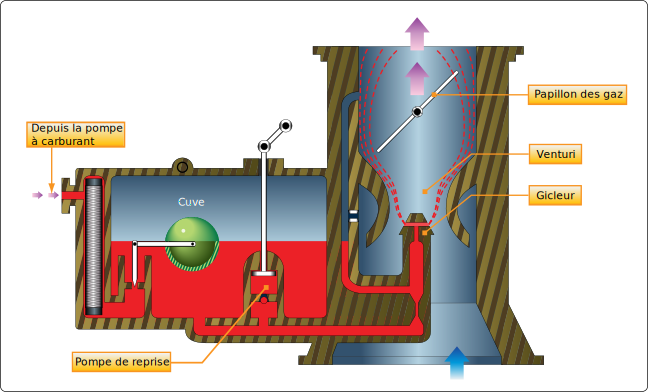
\includegraphics[width=0.5\textwidth]{01-EtudeAeronefs/img/systemesAvion/carburateur.pdf}
  		\legende{Schéma d'un carburateur}{img:carburateur}
	\end{figure}	
	
	Le carburateur dispose d'un petit réservoir appelé cuve, dans lequel le niveau de carburant, en provenance des réservoirs et mis en pression grâce à des pompes, est maintenu constant grâce à un flotteur qui commande l'ouverture d'un pointeau.
	
	Un dispositif appelé pompe de reprise, actionné mécaniquement lorsque la manette des gaz est avancée rapidement, permet d'envoyer dans le carburateur une quantité supplémentaire de carburant lorsque le pilote demande une augmentation rapide de la puissance. Cela permet d'aider le moteur à atteindre rapidement le régime demandé par le pilote.
	
	\subparagraph{Givrage carburateur}
	Au sein du carburateur, le tube Venturi est le siège d'une dépression. Comme toute baisse de pression, elle s'accompagne d'une baisse de la température. Cette baisse est suffisante pour atteindre le point de condensation puis de congélation de la vapeur d'eau présente dans l'air.
	
	Le carburateur peut alors subir un givrage : de la glace se forme dans le carburateur, ce qui va provoquer la réduction du passage disponible pour l'air. Cela peut aboutir, si rien n'est fait et que la situation est maintenue, à une réduction telle du passage de l'air que le moteur s'arrêtera.
	
	\begin{figure}[H]
  		\centering
    		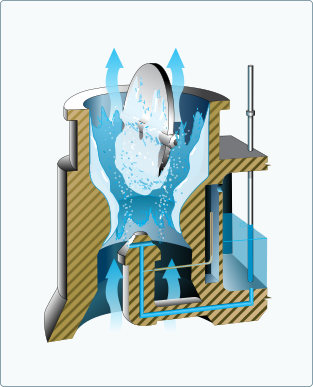
\includegraphics[width=0.25\textwidth]{01-EtudeAeronefs/img/systemesAvion/givrageCarbu.pdf}
  		\legende{Illustration d'un givrage carburateur}{img:givrageCarbu}
	\end{figure}
	
	Pour pallier à ce risque, les moteurs à carburateurs sont généralement équipés de système de réchauffage du carburateur. On réchauffe à cette fin de l'air en la faisant passer autour du pot d'échappement. L'air présenté en entrée du carburateur est ainsi suffisamment chaud pour que la chute de la température dans le carburateur ne présente plus de risque d'atteinte du point de congélation.
	
	\begin{figure}[H]
  		\centering
    		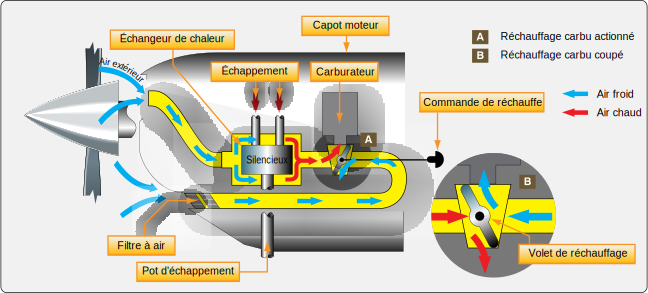
\includegraphics[width=0.85\textwidth]{01-EtudeAeronefs/img/rechauffeCarbu.pdf}
  		\legende{Illustration d'un givrage carburateur}{img:rechauffeCarbu}
	\end{figure}
	
	Ce réchauffage du carburateur n'est cependant utilisé que lorsqu'il est strictement nécessaire (faible régime) car l'air plus chaud étant moins dense, l'usage du réchauffage carburateur provoque une réduction de la puissance délivrée par le moteur. En effet, l'air chaud étant moins dense, la quantité d'oxygène disponible pour la combustion s'en trouve réduite.
	
	
	\subsection{Motorisation électrique}
	
	\subsection{Turbopropulseurs et turbomoteurs}
	\begin{figure}[H]
  	\centering
    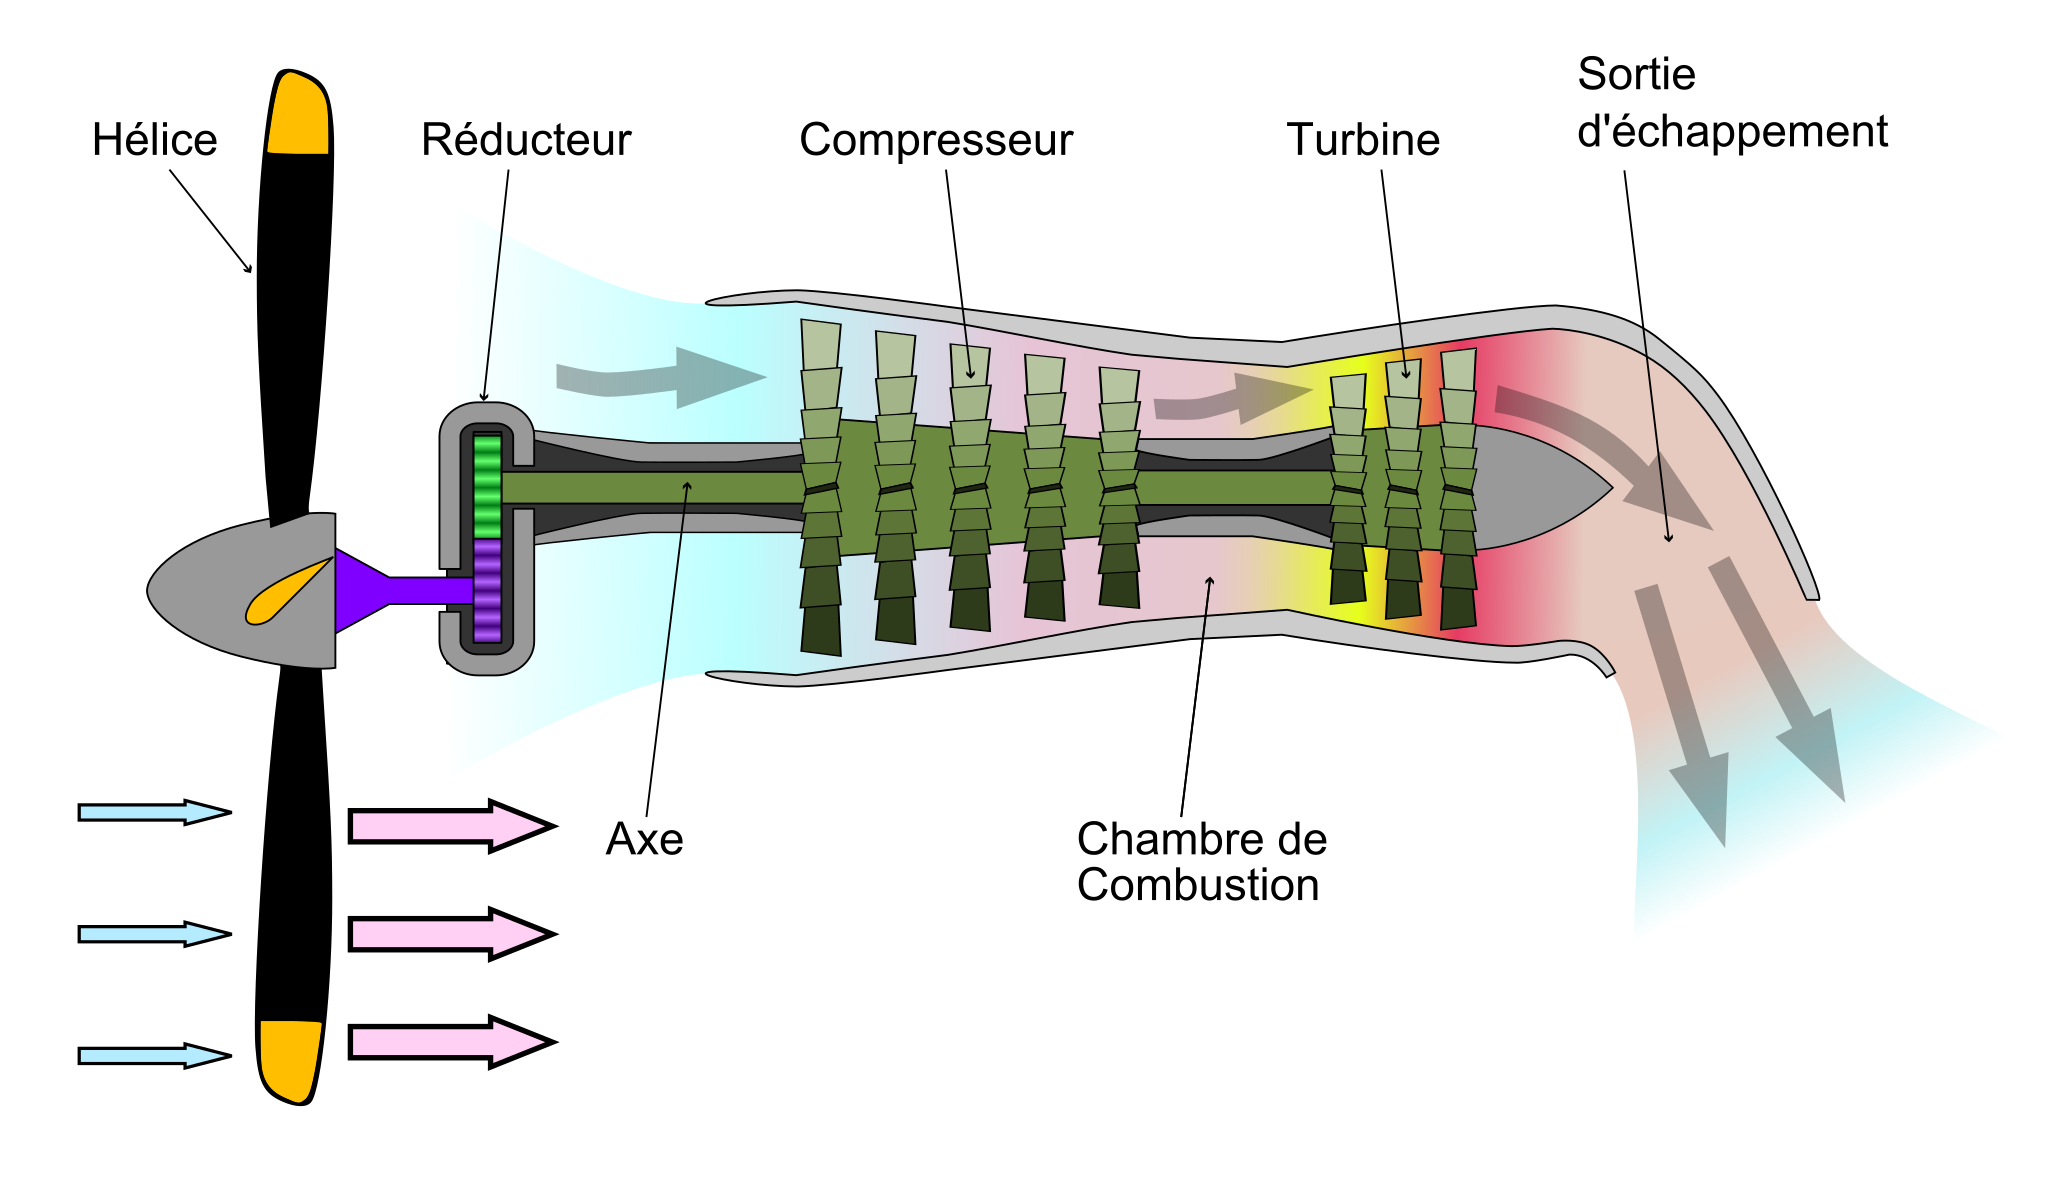
\includegraphics[width=0.75\textwidth]{01-EtudeAeronefs/img/turbomachines/turbopropulseur.pdf}
  	\legende{Schéma d'un turbopropulseur}{img:turbopropulseur}
	\end{figure}	
	
	\subsection{Hélices et moteurs}
	
	\subsection{Propulseurs à réaction}
		\subsubsection{Turboréacteurs}
		\begin{figure}[H]
  		\centering
    		\includegraphics[width=0.75\textwidth]{01-EtudeAeronefs/img/turbomachines/turboreacteur-schema.pdf}
  		\legende{Schéma de fonctionnement d'un turboréacteurs simple flux}{img:turboreacteur-schema}
		\end{figure}			
		
		
		\begin{figure}[H]
  		\centering
    		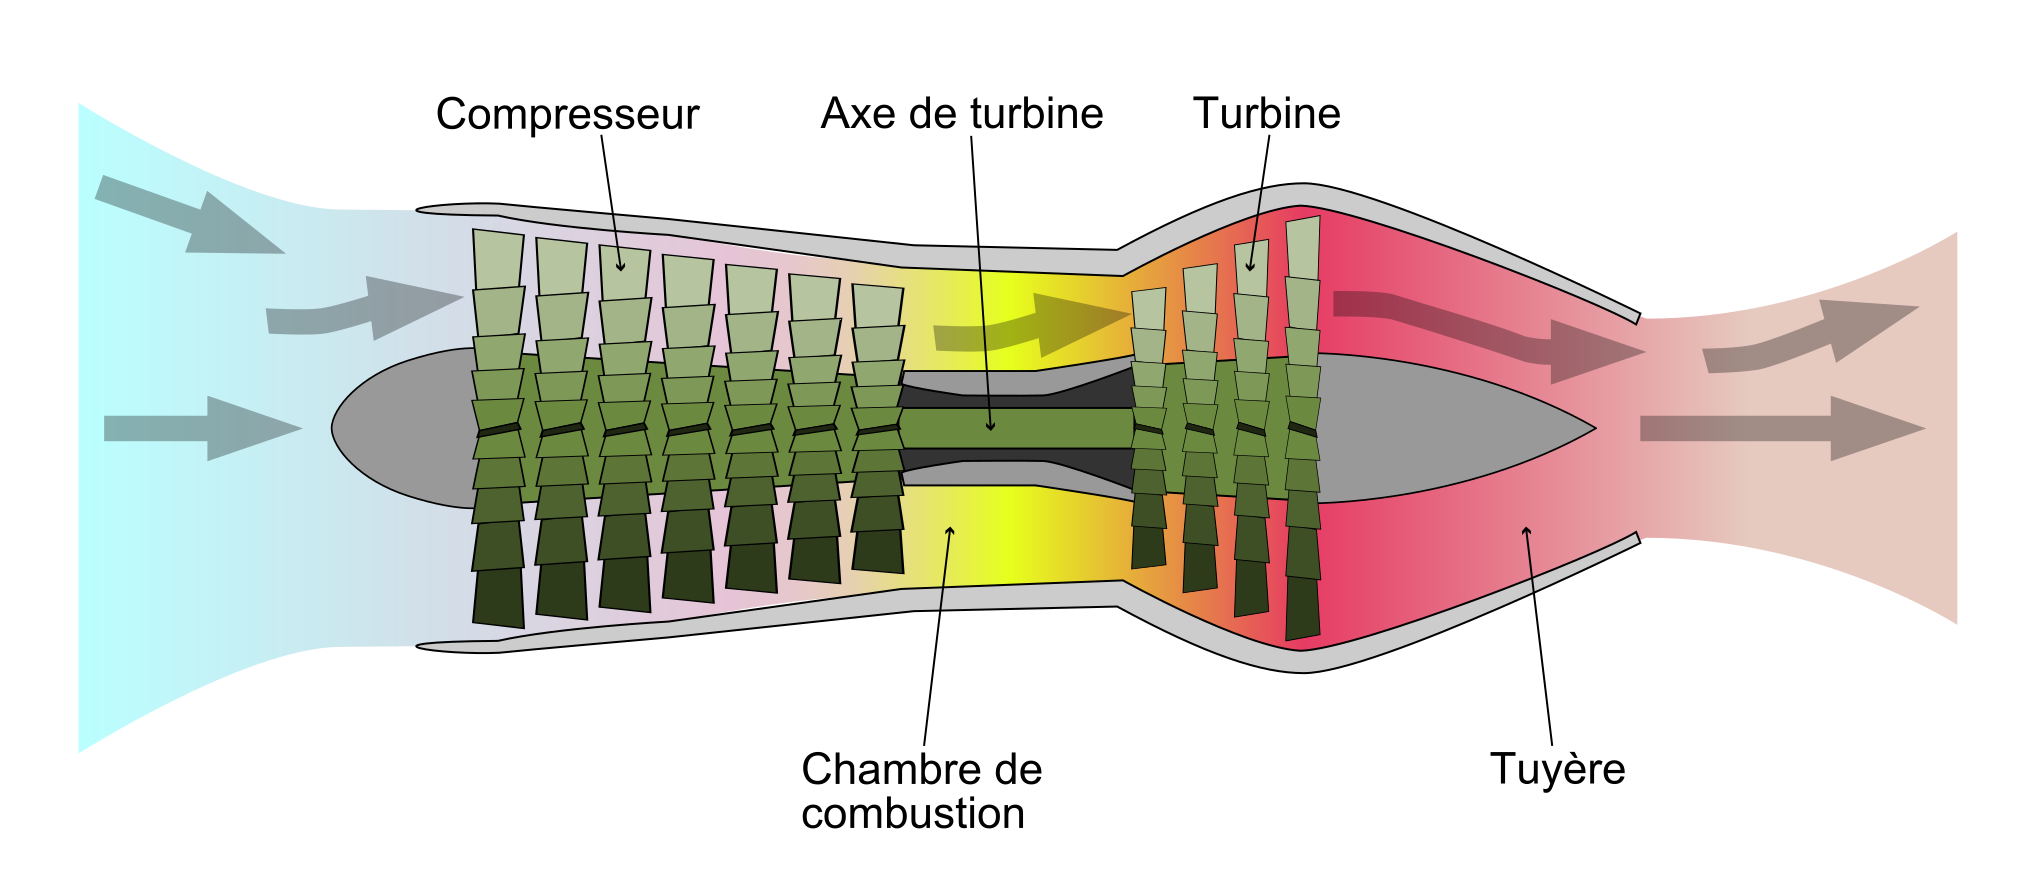
\includegraphics[width=0.75\textwidth]{01-EtudeAeronefs/img/turbomachines/turboreacteur-simpleFlux.pdf}
  		\legende{Schéma d'un turboréacteurs simple flux}{img:turboreacteur-simpleFlux}
		\end{figure}	
	
		\begin{figure}[H]
  		\centering
    		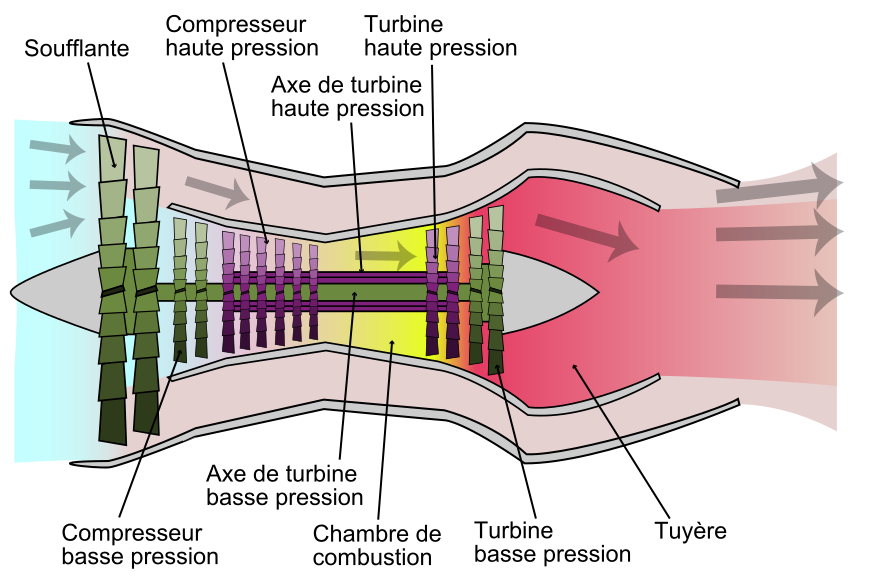
\includegraphics[width=0.75\textwidth]{01-EtudeAeronefs/img/turbomachines/turboreacteur-doubeFlux.pdf}
  		\legende{Schéma d'un turboréacteurs double flux}{img:turboreacteur-doubeFlux}
		\end{figure}	
	
		\subsubsection{Statoréacteurs}
	
		\subsubsection{Moteurs fusées}
		
	\subsection{Contraintes liées au développement durable}
